The implementation of the tools and the subsequent comparison is done using the following steps in the following order:
\begin{itemize}
    \item Export all \coq objects from the standard library and the selected corpora.
    \item Distinguish theorems from other definitions.
    \item Generate a \dagraph of dependencies for all \coq objects.
    \item Select and extract various features.
    \item Select and perhaps combine various \machinelearning methods.
    \item Analyse which combination of features and \machinelearning methods work best for which corpus, and how well these configurations generalize.
\end{itemize}

The selection of features and \machinelearning techniques will occur during the research itself.
The corpora used are determined beforehand.

\begin{figure}[H]
	\centering
	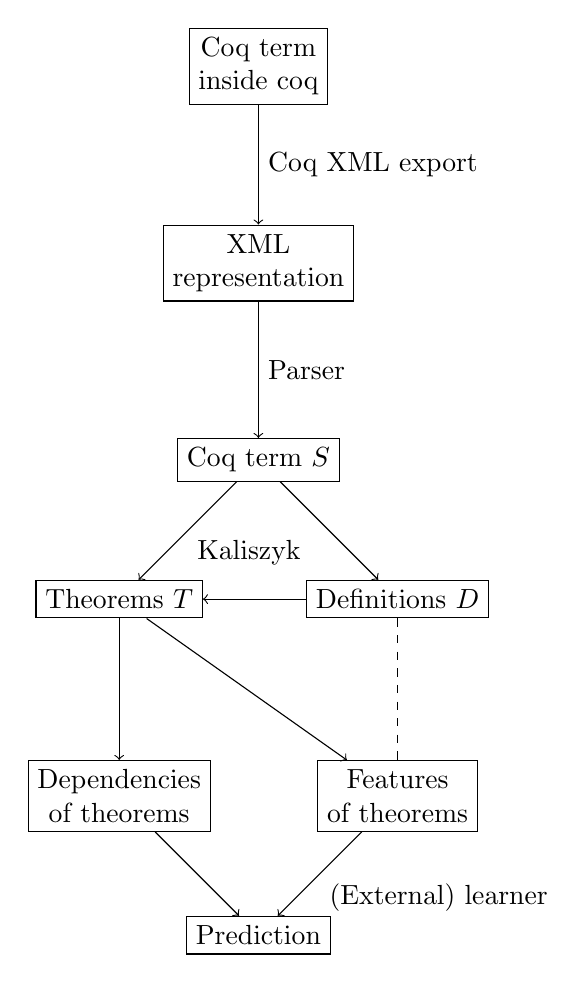
\begin{tikzpicture}[auto, node distance=2.5cm, main/.style={draw,align=center}]
		\node[main] (coq) {Coq term\\inside coq};
		\node[main] (xml) [below of=coq] {XML\\representation};
		\node[main] (term) [below of=xml] {Coq term $S$};
		\node[main] (definitions) [below right of=term] {Definitions $D$};
		\node[main] (theorems) [below left of=term] {Theorems $T$};
		\node[main] (features) [below of=definitions] {Features\\of theorems};
		\node[main] (dependencies) [below of=theorems] {Dependencies\\of theorems};
		\node[main] (prediction) [below left of=features] {Prediction};

		\path [->]
			(coq) edge node {Coq XML export} (xml)
			(xml) edge node {Parser} (term)
			(term) edge node {} (definitions)
			(term) edge node {Kaliszyk} (theorems)
			(definitions) edge node {} (theorems)
			(theorems) edge node {} (features)
			(theorems) edge node {} (dependencies)
			(features) edge node {(External) learner} (prediction)
			(dependencies) edge node {} (prediction);
		
		\draw [dashed] (definitions) -- (features);
	\end{tikzpicture}
	\caption{Transformations performed by the \premiseselection tooling.}
\end{figure}


\subsection{Tooling}
Various design goals of the \premiseselection tool are to:
\begin{itemize}
    \item Support offline learning and analysis of \machinelearning on the various corpora.
    \item Enable integration in the \coqide GUI.
    	I would like to create something like Clippy or Vigor for \coq.
    \item Enable merging of the premise selection tool in the \coq main branch as a plugin.
\end{itemize}
In order to achieve this, I decided to implement the tool on top of the \acic datastructures
as exported by the \xml plugin in \coq.
As far as reasonable the \premiseselection tooling will be written in \ocaml.
I foresee that some effort will be required to interface \ocaml with existing implementations
of canonical \machinelearning algorithms.
The \machinelearning field favours \python and \matlab as the preferred development environments.
Ideally the tooling created can be used as a building block in a future \coq tactic which finishes proofs fully automatically.

\subsection{Extraction}
The \coq XML plugin exports various objects.
After parsing the XML output only some of these constructs are used.
Of these, the following \coq objects are used:
\begin{description}
    \item[(Co)Inductive definitions]
        \coq allows for (co)inductive definitions.
        These definitions are composed of a name, a type, and a list of constructors.
        Each constructor also is composed of a name and a type.
        A constructor is a valid definition which can be used in theorems.
		A (Co)Inductive definition also yields an induction principle (\texttt{ind}) and a recursion scheme (\texttt{rec}).
		These are also separately exported by \coq, and thus need not be considered further.

    \item[Constants (definitions / theorems / axioms)]
        The types and bodies of constants are defined separately, as needed.
        Theorems are proof-irrelevant, whilst definitions need to be substituted when applied.
        These objects they become undistinguishable when exported.
        Axioms only generate a type, and no body.
\end{description}

If time permits, also the following objects could be used:
\begin{description}
    \item[Proof in progress]
        Consists of a name, a type, a body and a list of dependencies.
        These dependencies still need to be satisfied to complete the proof.
    \item[Tactics application]
        On a higher level, tactics can be applied in order to form a proof.
        These higher level constructs are dependant on the proof engine.
        A proof consisting of tactics can thus become invalid given another \coq version.
        For premise selection these tactics can help solve proofs more quickly, because the proofs they form are smaller.
\end{description}

\coq also exports variables, but these are not used.
A variable consists of a name and a type, and becomes a parameter when a theory which uses the variable is applied.
Thusfar there is no use for these variables within this project.

\subsection{Features and output}
When performing \premiseselection, only theorems are regarded.
For other definitions selecting premises is conceptually problematic.
As the training set, for each proven theorem the features are computed from the type.
The definitions used in the body of a theorem are the desired result of the \premiseselection.
Hence, given the type of a new theorem to be proved, the \premiseselection yields a set of definitions which are likely to help prove the theorem.
These definitions are ordered by the chance the definition can be used in the proof.
This ordering is derived from the used definitions of similar complete theorems.
The similarity of complete theorems is captured in the model employed in the \premiseselection, and is derived from the features.

Distinguishing theorems from other definitions is not trivial.
Normally only definitions of kind \prop need to be considered as theorems.
However in the case of \corn the propositions are of type \cprop, which is of kind \kindtype.
Also the kind of a definition is not exported consistently by \coq.
Instead I will initially use a heuristic as defined by Kaliszyk \cite{kaliszyk2014machine}.
This heuristic defines the theorems, or the set of allowed dependencies, as all definitions except those used in the types of definitions.

For the prototype only the definitions used in the theorem type are regarded as features.
Concretely, for a set of proven theorems with their types and bodies, the used definitions from the types are collected.
For this set of proven theorems, a feature matrix $F$ is constructed.
The \texttt{true} boolean value $F_{ij}$ then represents the usage of definition $j$ in the type of the proven theorem $i$.

For the body of each proven theorem the used definitions are similarly collected, and a dependency matrix $D$ is constructed.
This matrix thus encodes the usage of definitions in the body of those proven theorems.

The predictor can now, for a unproven theorem, compute the features from the type and yield the ordered set of definitions likely to be useful in the to be constructed body.
After the prototype is completed additional features will be considered and implemented.
Most notably some corpus specific features will be tried.

\subsection{Types}
As a computer science student I like to give the transformations within the tool types:
\[
	\begin{array}{lclcl}
		\mathbf{depanalysis} & : & \text{aobj} & \longrightarrow & [\text{id} \times [\text{id}] \times [\text{id}]] \\
			& & \text{object} & \longmapsto & [\text{theorem} \times [\text{feature}] \times [\text{dependency}]]
	\end{array}
\]


\[
	\begin{array}{lclclcl}
		\mathbf{featuregen} & : & [\text{id}] & \times & [[\text{id}]] & \longrightarrow & 2^{\text{id} \times \text{id}} \\
			& & \text{all\_features} & \times & \text{features\_per\_theorem} & \longmapsto & \text{feature matrix}~F
	\end{array}
\]

Similarly \textbf{dependencygen}.

\[
	\begin{array}{lclclclcl}
		\mathbf{predict} & : & 2^{\text{id} \times \text{id}} & \times & 2^{\text{id} \times \text{id}} & \times & 2^{\text{id}} & \longrightarrow & [\text{id}] \\
			 & & \text{feature matrix}~F & \times & \text{dependency matrix}~D & \times & \text{feature vector}~V & \longmapsto & \text{prediction}
	\end{array}
\]

\subsection{Example}
\begin{lstlisting}[language=Coq, mathescape]
Inductive nat : Set :=
  | O : nat
  | S : nat -> nat.

Definition nat_id := $\ldots$ .

Fixpoint plus (n m : nat) : nat :=
  match n with
  | O => m
  | S p => S (p + m)
  end.

Lemma plus_0_r : $\forall$ x , plus x 0 = x.
Proof.
$\ldots$ nat_ind $\ldots$
Qed.
Definition plus_0_r n := eq_sym (nat_ind _ eq_refl $\ldots$ ).
\end{lstlisting}

\begin{lstlisting}[language=Coq, mathescape, frame=none]
$S = \{$
	nat : Set$,$
	O : nat$,$
	S : nat -> nat$,$
	nat_ind : $\forall$ P : nat -> Prop, P 0 -> ($\forall$ n : nat, P n -> P (S n)) -> $\forall$ n : nat, P n := fix $\ldots$$,$
	plus : nat -> nat -> nat := fix $\ldots$$,$
	plus_0_r : $\forall$ x , plus x 0 = x := $\ldots$ nat_ind $\ldots$ $,$
$\} $
\end{lstlisting}

\begin{lstlisting}[language=Coq, mathescape, frame=none]
$D = \{$nat$,$ 0$,$ S$,$ plus$\}$
\end{lstlisting}

\begin{lstlisting}[language=Coq, mathescape, frame=none]
$T = \mathtt{dom}(S) \setminus D = \{$nat_ind$,$ plus_0_r$\}$
\end{lstlisting}

\subsection{Corpora}
\begin{description}
    \item[\compcert]
    \item[\formalin]
    \item[\corn]
    \item[\mathcomp]
\end{description}

%\subsection{Metrics}
%The performance of a predictor is measured using \texttt{Recall}:


% Cross validation on Corpora
% `Proof in Progress` -> step (aconstr)
% Subset corpora (Train) -> Corpus (Test) -> Rating
% A corpus is divided into Proofs in Progress (each substep)
% Ratio of guessed steps 
